% !TEX program = xelatex
\documentclass[aspectratio=169, 12pt]{beamer}

% ── Theme ──────────────────────────────────────────────────────
\usetheme{metropolis}
\usepackage{appendixnumberbeamer}
\usepackage{booktabs}
\usepackage{amsmath, amssymb}
\usepackage{graphicx}
\usepackage{tikz}
\usetikzlibrary{arrows.meta, positioning, decorations.pathreplacing, calc}
\usepackage{pgfplots}
\pgfplotsset{compat=1.18}

% ── Colors (matched to compass-dark-swap.png) ─────────────────
\definecolor{accent}{HTML}{C84B31}    % warm amber-red from vintage maps
\definecolor{darkbg}{HTML}{1B2838}    % dark navy from compass shadow
\definecolor{midbg}{HTML}{4A6F8A}     % steel blue from map background
\definecolor{lightbg}{HTML}{7B9CB8}   % lighter steel blue
\definecolor{offwhite}{HTML}{E8E0D4}  % parchment / aged paper

\setbeamercolor{frametitle}{bg=darkbg, fg=offwhite}
\setbeamercolor{progress bar}{fg=accent}
\setbeamercolor{alerted text}{fg=accent}
\setbeamercolor{standout}{bg=darkbg, fg=offwhite}

% ── Compact frame titles ──────────────────────────────────────
\setbeamerfont{frametitle}{size=\normalsize}
\makeatletter
\setlength{\metropolis@frametitle@padding}{1.2ex}
\makeatother

% ── Metadata ───────────────────────────────────────────────────
\title{Cuando la IA Olvida lo que le Pediste}
\subtitle{Context Rot, Instruction Decay y por qu\'e importa}
\author{Tom\'as Pablo Korenblit}
\date{2026}
\institute{Licenciatura en Ciencia de Datos $\cdot$ Ciencia de Datos $\cdot$ 1C2026\\
Docentes: Rodrigo D\'iaz, Agust\'in Moro, Florencia Pi\~neyr\'ua}

\begin{document}

% ══════════════════════════════════════════════════════════════
% Custom title slide with compass background
{
\setbeamertemplate{footline}{}
\setbeamertemplate{navigation symbols}{}
\begin{frame}[plain]
\begin{tikzpicture}[remember picture, overlay]
    % Background image — fill entire page
    \node[anchor=center, inner sep=0pt, outer sep=0pt] at (current page.center) {%
        
\includegraphics[width=\the\paperwidth, height=\the\paperheight]{img/compass-dark-swap.png}};
    % Dark overlay for readability
    \fill[darkbg, opacity=0.6] (current page.south west) rectangle (current page.north east);
    % Title text — upper area
    \node[text width=12cm, align=center] at ([yshift=1.2cm]current page.center) {%
        {\color{offwhite}\LARGE\bfseries Cuando la IA Olvida\\[0.2em] lo que le Pediste}\\[0.8em]
        {\color{lightbg}\normalsize Context Rot, Instruction Decay y por qu\'e importa}
    };
    % Author info — lower area
    \node[text width=12cm, align=center] at ([yshift=-2cm]current page.center) {%
        {\color{offwhite}\normalsize Tom\'as Pablo Korenblit}\\[0.5em]
        {\color{lightbg}\footnotesize Licenciatura en Ciencia de Datos $\cdot$ Ciencia de Datos $\cdot$ 1C2026}\\[0.3em]
        {\color{lightbg}\footnotesize Docentes: Rodrigo D\'iaz, Agust\'in Moro, Florencia Pi\~neyr\'ua}
    };
\end{tikzpicture}
\end{frame}
}

% ══════════════════════════════════════════════════════════════
% (a) HOOK
% ══════════════════════════════════════════════════════════════

\begin{frame}{}

\vspace{1em}

\Large
Est\'as usando ChatGPT.

\vspace{0.3em}

\normalsize
Le explic\'as tu proyecto, le ped\'is que siga ciertas reglas, y funciona b\'arbaro. Van y vienen mensajes. Todo bien.

\vspace{1.5em}
\pause

\Large
Hasta que en el mensaje 15\ldots

\vspace{0.3em}

\normalsize
te responde cualquier cosa, como si nunca le hubieras dicho nada.

\vspace{1.5em}
\pause

\Large
\alert{¿Qu\'e pas\'o?}

\end{frame}

% ══════════════════════════════════════════════════════════════
% (b) THE FIELD — Biology of an LLM
% ══════════════════════════════════════════════════════════════
\section{El Campo: ¿C\'omo Funciona un LLM?}

% ══════════════════════════════════════════════════════════════
\begin{frame}{Un LLM es una M\'aquina de Predicci\'on}

Un Large Language Model no ``entiende''. Predice: dado todo lo anterior, ¿qu\'e palabra viene?

\vspace{1em}

Pero esa predicci\'on es sofisticada. El a\~no pasado, Anthropic le hizo reverse engineering a uno de sus modelos y public\'o lo que encontr\'o adentro (Lindsey et al., 2025):

\vspace{1em}

\begin{itemize}
    \item No procesa paso a paso. Eval\'ua \textbf{m\'ultiples caminos en paralelo} y ``vota''
    \item Planifica hacia adelante: elige una palabra futura \emph{antes} de escribir lo que viene antes
\end{itemize}

\vspace{1em}

¿C\'omo lo hace? Con \textbf{circuitos internos}.

\end{frame}

% ══════════════════════════════════════════════════════════════
\begin{frame}{Circuitos internos}

\begin{columns}[c]
\begin{column}{0.35\textwidth}
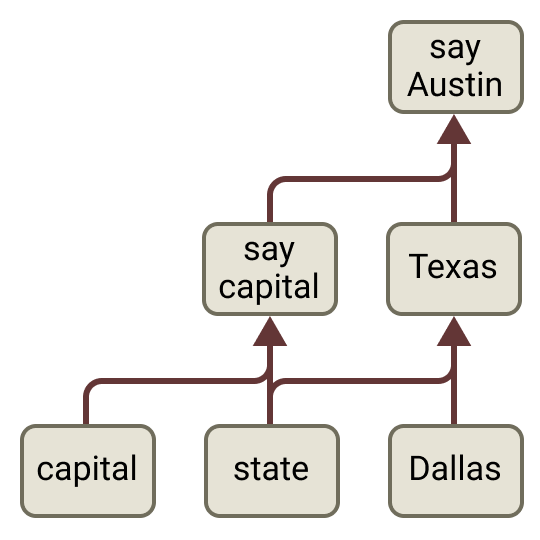
\includegraphics[width=\textwidth]{img/anthropic-multi-step-reasoning-circuit.png}
\end{column}

\begin{column}{0.60\textwidth}
\emph{``¿Cu\'al es la capital del estado donde est\'a Dallas?''}

\vspace{0.8em}

El modelo encadena representaciones internas:

\vspace{0.3em}

\textbf{Dallas} $\to$ \textbf{Texas} $\to$ \textbf{capital} $\to$ \textbf{Austin}

\vspace{0.8em}

Cada nodo es una \emph{representaci\'on interna} (no confundir con feature de un dataset) que se activa seg\'un el contexto.

\vspace{0.5em}

{\footnotesize Lindsey et al., 2025. Transformer Circuits.}
\end{column}
\end{columns}

\end{frame}

% ══════════════════════════════════════════════════════════════
\begin{frame}{La atenci\'on: lo que el modelo ``mira''}

Para generar cada palabra, el modelo decide \textbf{a qu\'e parte del texto prestarle atenci\'on}.

\vspace{0.7em}

Funciona bien cuando el contexto es corto: hay pocos tokens y el modelo puede atender a cada uno.

\vspace{0.7em}

Pero la atenci\'on es un \textbf{recurso finito}. Se reparte entre \emph{todos} los tokens del contexto. Cuando el contexto crece, las instrucciones del principio tienen que competir con todo lo que vino despu\'es.

\vspace{1em}

\begin{center}
\large
¿Qu\'e pasa cuando hay \alert{\textbf{un mill\'on de tokens}} compitiendo por atenci\'on?
\end{center}

\end{frame}

% ══════════════════════════════════════════════════════════════
\begin{frame}{La Ventana de Contexto}

\begin{columns}[T]
\begin{column}{0.55\textwidth}
\textbf{Token} = la unidad m\'inima que procesa el modelo.\\
Una palabra $\approx$ 1--2 tokens. Una p\'agina $\approx$ 500.

\vspace{1em}

\textbf{Ventana de contexto} = todo lo que el modelo puede ``ver'' al responder: el system prompt, la conversaci\'on, los archivos.

\vspace{1em}

Si algo \textbf{no est\'a en la ventana}, el modelo \textbf{no lo sabe}. No tiene memoria aparte.
\end{column}

\begin{column}{0.42\textwidth}
\renewcommand{\arraystretch}{1.3}
\begin{tabular}{@{} l r @{}}
\toprule
\textbf{A\~no} & \textbf{Contexto} \\
\midrule
2023 & 4K--16K \\
2024 & 128K--200K \\
2025 & 200K \\
2026 & \alert{\textbf{1M tokens}} \\
\bottomrule
\end{tabular}

\vspace{0.8em}
\footnotesize
1M tokens $\approx$ 2.000 p\'aginas.\\[0.3em]
M\'as ventana deber\'ia ser mejor, ¿no?
\end{column}
\end{columns}

\end{frame}

% ══════════════════════════════════════════════════════════════
\begin{frame}{System prompt y guardrails}

\begin{columns}[c]
\begin{column}{0.57\textwidth}
\textbf{System prompt} = instrucciones que recibe el modelo \emph{antes} de hablar con el usuario.

\vspace{0.5em}

\begin{itemize}
    \item \textbf{Formato} --- ``respond\'e en espa\~nol''
    \item \textbf{Persona} --- ``sos un tutor amable''
    \item \textbf{Seguridad} --- ``no generes contenido da\~nino''
    \item \textbf{L\'ogica} --- ``us\'a tal herramienta para tal tarea''
\end{itemize}

\vspace{0.5em}

Los \textbf{guardrails} no son un m\'odulo especial.\\
Son instrucciones como cualquier otra.
\end{column}

\begin{column}{0.38\textwidth}
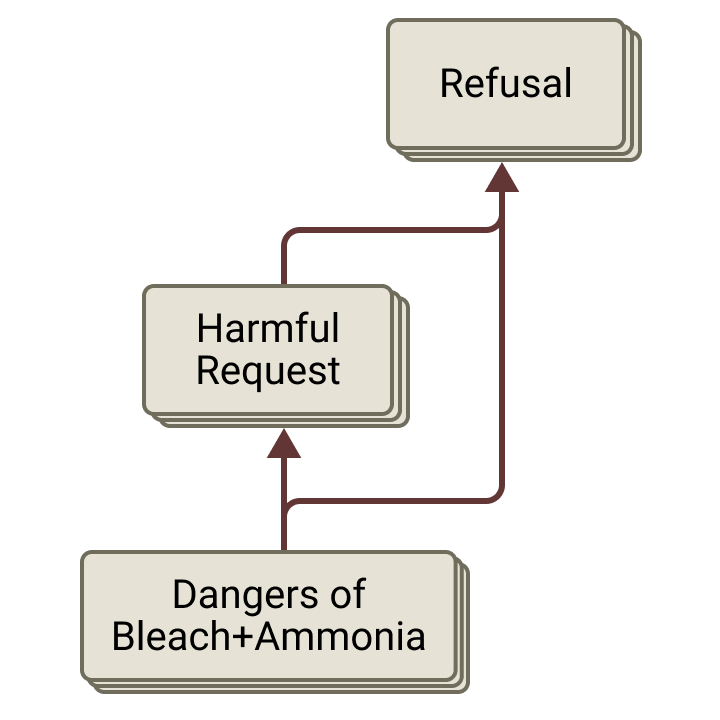
\includegraphics[width=\textwidth]{img/anthropic-refusal-circuit.png}

\vspace{0.3em}
{\scriptsize La seguridad es un \emph{pathway}, no un interruptor. (Lindsey et al., 2025)}
\end{column}
\end{columns}

\end{frame}

% ══════════════════════════════════════════════════════════════
% (d) SHOW DEGRADATION
% ══════════════════════════════════════════════════════════════
\section{El Problema: Context Rot}

% ══════════════════════════════════════════════════════════════
\begin{frame}{La Evidencia}

\begin{center}
\renewcommand{\arraystretch}{1.5}
\begin{tabular}{@{} p{7.5cm} r l @{}}
\toprule
\textbf{Hallazgo} & \textbf{N\'umero} & \textbf{Fuente} \\
\midrule
Ca\'ida en tareas multi-turn & \alert{\textbf{39\%}} & Laban et al., 2025 \\
Accuracy en 3 turnos: 87.7\% $\to$ & \alert{\textbf{70.7\%}} & He et al., 2024 \\
Modelos frontera donde se observa & \alert{\textbf{18/18}} & Chroma, 2025 \\
Con 50+ reglas, adherencia $\to$ & \alert{\textbf{$\sim$0\%}} & Mu et al., 2025 \\
\bottomrule
\end{tabular}
\end{center}

\vspace{1em}

\begin{center}
\footnotesize
No es un bug de un modelo. Le pasa a \textbf{todos}: los 18 modelos frontera testeados.
\end{center}

\end{frame}

% ══════════════════════════════════════════════════════════════
\begin{frame}{¿Por qu\'e pasa? La Curva U}

\begin{center}
\begin{tikzpicture}
\begin{axis}[
    width=11cm, height=5cm,
    xlabel={Posici\'on de la informaci\'on en el contexto},
    ylabel={Precisi\'on (\%)},
    xmin=0, xmax=10, ymin=40, ymax=100,
    xtick={0, 5, 10},
    xticklabels={Inicio, Medio, Final},
    ytick={40, 60, 80, 100},
    grid=major,
    grid style={gray!20},
    thick,
    axis lines=left,
]
\addplot[color=accent, ultra thick, smooth, tension=0.6]
    coordinates {(0,90) (1,85) (2,72) (3,58) (4,50) (5,48)
                 (6,50) (7,58) (8,72) (9,85) (10,92)};
\node[fill=white, draw=accent, rounded corners, inner sep=4pt]
    at (axis cs:5,68) {\footnotesize \textbf{Zona de olvido}};
\draw[-{Stealth}, accent, thick] (axis cs:5,65) -- (axis cs:5,51);
\end{axis}
\end{tikzpicture}
\end{center}

\vspace{0.3em}

Liu et al.\ (2023) midi\'o esto en tareas de recuperaci\'on de informaci\'on. El patr\'on sugiere que la atenci\'on no es uniforme, lo que podr\'ia explicar por qu\'e las instrucciones tambi\'en se pierden.

\end{frame}

% ══════════════════════════════════════════════════════════════
\begin{frame}{¿Y por qu\'e deber\'ia importarnos?}

\begin{columns}[T]
\begin{column}{0.48\textwidth}
\textbf{Plata:}
\begin{itemize}
    \item Empresas procesan \textbf{miles de millones} de tokens por d\'ia
    \item Cada token de reminder cuesta
    \item Refuerzo ineficiente $\times$ esa escala = mucha plata
\end{itemize}
\end{column}

\begin{column}{0.48\textwidth}
\textbf{Seguridad:}
\begin{itemize}
    \item Los guardrails son instrucciones como cualquier otra
    \item \textbf{Hip\'otesis:} seguridad podr\'ia decaer m\'as r\'apido que formato
    \item Si es as\'i, los reminders uniformes \alert{sub-invierten en seguridad}
\end{itemize}
\end{column}
\end{columns}

\vspace{0.5em}

\footnotesize
Le ped\'is que solo cite fuentes reales. 10 turnos despu\'es, te inventa un paper que no existe.

\end{frame}

% ══════════════════════════════════════════════════════════════
\begin{frame}{¿Qu\'e se Hace Hoy?}

\renewcommand{\arraystretch}{1.4}
\begin{table}
\centering
\footnotesize
\begin{tabular}{@{} p{3.5cm} p{4.5cm} p{4.2cm} @{}}
\toprule
\textbf{Estrategia} & \textbf{Idea} & \textbf{Problema} \\
\midrule
Repetir todo, siempre &
    Re-inyectar el prompt completo cada turno &
    Saturaci\'on: m\'as reglas $\to$ \emph{menos} adherencia \\

Duplicar el prompt &
    Poner las instrucciones dos veces (Google, 2025) &
    2$\times$ costo en tokens \\

No hacer nada &
    Confiar en que el modelo recuerda &
    39\% de ca\'ida documentada \\

Jerarqu\'ia de prioridad &
    System $>$ User (OpenAI, 2024) &
    No aborda el decaimiento gradual \\
\bottomrule
\end{tabular}
\end{table}

\vspace{0.8em}

\begin{center}
Ninguna es \textbf{adaptativa}. \alert{Ninguna decide \emph{qu\'e} reforzar ni \emph{cu\'ando}.}
\end{center}

\end{frame}

% ══════════════════════════════════════════════════════════════
% (g) THE KEY QUESTION
% ══════════════════════════════════════════════════════════════
\begin{frame}{La Pregunta Clave}

\begin{center}
\Large
Si sabemos que el modelo \textbf{olvida}\ldots\\[0.5em]
y sospechamos que cada instrucci\'on \textbf{decae distinto}\ldots\\[1em]
\pause
¿por qu\'e reforzamos \textbf{todo por igual}?\\[1.5em]
\pause
\normalsize
¿Y si pudi\'eramos reforzar \alert{\textbf{solo lo que se est\'a por olvidar}}?
\end{center}

\end{frame}

% ══════════════════════════════════════════════════════════════
% (h) BAYESIAN THINKING
% ══════════════════════════════════════════════════════════════
\section{Una Direcci\'on: Pensar Bayesianamente}

% ══════════════════════════════════════════════════════════════
\begin{frame}{Pensar en Probabilidades, No en Reglas}

\begin{columns}[T]
\begin{column}{0.48\textwidth}
\textbf{Enfoque cl\'asico:}\\[0.3em]
``¿Cumple o no cumple?'' --- binario.\\[0.5em]
Si cumple, no hacemos nada.\\
Si no cumple, ya es tarde.\\[1em]
No distingue entre una instrucci\'on que est\'a al 90\% y una al 51\%.
\end{column}

\begin{column}{0.48\textwidth}
\textbf{Enfoque Bayesiano:}\\[0.3em]
Mantenemos un \emph{posterior} para cada instrucci\'on.\\[0.5em]
Cada observaci\'on \textbf{actualiza} la estimaci\'on (verosimilitud $\times$ prior).\\[0.5em]
Entre turnos, el posterior \textbf{decae} naturalmente.\\[0.5em]
Podemos \textbf{anticipar} el olvido antes de que pase.
\end{column}
\end{columns}

\end{frame}

% ══════════════════════════════════════════════════════════════
\begin{frame}{Bayesian Knowledge Tracing (BKT)}

BKT se usa hace 30 a\~nos en educaci\'on: estima la probabilidad de que un \textbf{estudiante} domine un concepto, turno a turno.

\vspace{0.8em}

\begin{center}
\begin{tikzpicture}[
    node distance=0.6cm and 2cm,
    box/.style={draw, rounded corners, minimum width=2.5cm, minimum height=0.8cm,
                align=center, font=\footnotesize},
    arr/.style={-{Stealth}, thick},
]
\node[box, fill=lightbg] (obs) {Observaci\'on\\{\scriptsize ¿Cumple la instrucci\'on?}};
\node[box, fill=offwhite, right=2.5cm of obs] (update) {Actualizaci\'on\\{\scriptsize Bayes update}};
\node[box, fill=accent!20, right=2.5cm of update] (belief) {Creencia\\{\scriptsize $P(\text{compliance}_i)$}};
\node[box, fill=darkbg, text=white, below=1cm of update] (decay) {Decaimiento\\{\scriptsize $\gamma < 1$ entre turnos}};

\draw[arr] (obs) -- (update);
\draw[arr] (update) -- (belief);
\draw[arr] (decay) -- (update);
\draw[arr, dashed, midbg] (belief.south) -- ++(0,-0.5) -| (obs.south);
\end{tikzpicture}
\end{center}

\vspace{0.8em}

\large
¿Qu\'e pasa si el ``estudiante'' es el \textbf{LLM} y los ``conceptos'' son sus \textbf{instrucciones}?

\end{frame}

% ══════════════════════════════════════════════════════════════
\begin{frame}{Modelando el olvido}

Para cada instrucci\'on $i$ en el turno $t$:

\[
P(C_i \mid \mathcal{O}_{1:t}) =
    \frac{P(\mathcal{O}_t \mid C_i) \cdot \overbrace{P(C_i \mid \mathcal{O}_{1:t-1})}^{\text{lo que cre\'iamos antes}}}
         {P(\mathcal{O}_t)}
\]

\begin{itemize}
    \item $C_i$ = la instrucci\'on $i$ sigue siendo cumplida
    \item $\gamma < 1$ controla cu\'anto decae entre turnos
    \item Con presupuesto fijo de $B$ tokens, se refuerzan solo las instrucciones con menor $P(C_i)$
\end{itemize}

\vspace{0.5em}

\begin{center}
\footnotesize
Nadie aplic\'o BKT a compliance de LLMs, ni midi\'o curvas de olvido por tipo de instrucci\'on,\\
ni optimiz\'o qu\'e reforzar con un presupuesto limitado de tokens.
\end{center}

\end{frame}

% ══════════════════════════════════════════════════════════════
\begin{frame}[standout]

\Large
¿Preguntas?

\end{frame}

% ══════════════════════════════════════════════════════════════
\appendix

\begin{frame}{Referencias}

\scriptsize
\begin{columns}[T]
\begin{column}{0.48\textwidth}

Lindsey et al.\ (2025). \emph{On the Biology of a Large Language Model}. Transformer Circuits.\par\medskip
Ameisen et al.\ (2025). \emph{Circuit Tracing}. Transformer Circuits.\par\medskip
Anthropic (2025). \emph{Activation Oracles}. alignment.anthropic.com.\par\medskip
Liu et al.\ (2024). \emph{Lost in the Middle}. TACL.\par\medskip
Chroma Research (2025). \emph{Context Rot}.\par\medskip
Du et al.\ (2025). \emph{Context Length Alone Hurts}. EMNLP.\par

\end{column}

\begin{column}{0.48\textwidth}

Laban et al.\ (2025). \emph{LLMs Get Lost in Multi-Turn Conversation}.\par\medskip
He et al.\ (2024). \emph{Multi-IF}. Meta.\par\medskip
Mu et al.\ (2025). \emph{System Prompt Robustness}.\par\medskip
Zhang \& Yang (2025). \emph{LLMs as Discounted Bayesian Filters}.\par\medskip
Google Research (2025). \emph{Prompt Repetition Improves Non-Reasoning LLMs}.\par\medskip
Wallace et al.\ (2024). \emph{The Instruction Hierarchy}. OpenAI.\par

\end{column}
\end{columns}

\end{frame}

\end{document}
